%%%%%%%%%%%%%%%%%%%%%%%%%%%%%%%%%%%%%%%%%
% Thesis 
% LaTeX Template
% Version 1.4 (30/6/13)
%
% This template has been downloaded from:
% http://www.latextemplates.com
%
% Original authors:
% Steven Gunn 
% http://users.ecs.soton.ac.uk/srg/softwaretools/document/templates/
% and
% Sunil Patel
% http://www.sunilpatel.co.uk/thesis-template/
%
% License:
% CC BY-NC-SA 3.0 (http://creativecommons.org/licenses/by-nc-sa/3.0/)
%
% Note:
% Make sure to edit document variables in the Thesis.cls file
%
%%%%%%%%%%%%%%%%%%%%%%%%%%%%%%%%%%%%%%%%%

%----------------------------------------------------------------------------------------
%	PACKAGES AND OTHER DOCUMENT CONFIGURATIONS
%----------------------------------------------------------------------------------------

\PassOptionsToPackage{pdftex}{graphicx}   % <---- Added by Lau to be able to use .eps figures

\documentclass[11pt, a4paper, oneside]{Thesis} % Paper size, default font size and one-sided paper

\graphicspath{{./Pictures/}} % Specifies the directory where pictures are stored

\usepackage[square, numbers, comma, sort&compress]{natbib} % Use the natbib reference package - read up on this to edit the reference style; if you want text (e.g. Smith et al., 2012) for the in-text references (instead of numbers), remove 'numbers' 
\usepackage{hhline}  % Added by Lau for double lines in tables
\hypersetup{urlcolor=blue, colorlinks=true} % Colors hyperlinks in blue - change to black if annoying
\title{\ttitle} % Defines the thesis title - don't touch this

\begin{document}

\frontmatter % Use roman page numbering style (i, ii, iii, iv...) for the pre-content pages

\setstretch{1.3} % Line spacing of 1.3

% Define the page headers using the FancyHdr package and set up for one-sided printing
\fancyhead{} % Clears all page headers and footers
\rhead{\thepage} % Sets the right side header to show the page number
\lhead{} % Clears the left side page header

\pagestyle{fancy} % Finally, use the "fancy" page style to implement the FancyHdr headers

\newcommand{\HRule}{\rule{\linewidth}{0.5mm}} % New command to make the lines in the title page
\newcommand{\angstrom}{\mbox{\normalfont\AA}}

% PDF meta-data
\hypersetup{pdftitle={\ttitle}}
\hypersetup{pdfsubject=\subjectname}
\hypersetup{pdfauthor=\authornames}
\hypersetup{pdfkeywords=\keywordnames}

%----------------------------------------------------------------------------------------
%	TITLE PAGE
%----------------------------------------------------------------------------------------

\begin{titlepage}
\begin{center}

\textsc{\LARGE \univname}\\[1.5cm] % University name
\textsc{\Large Algorithm Engineering}\\[0.5cm] % Thesis type

\HRule \\[0.4cm] % Horizontal line
{\huge \bfseries \ttitle}\\[0.4cm] % Thesis title
\HRule \\[1.5cm] % Horizontal line
 
\large\emph{Authors:}\\[1cm]

\begin{minipage}{0.3\textwidth}
\begin{flushleft} \normalsize
{Laurids Møller Jepsen
\\ XXXXXXXX
\\ {\tiny laurids.mj@gmail.com}
}
\end{flushleft}
\end{minipage}
\begin{minipage}{0.3\textwidth}\normalsize\center
{Jeppe Haugaard Sørensen
\\ XXXXXXXX
\\ {\tiny jeppe.haugaard.sorensen@gmail.com}
}
\end{minipage}
\begin{minipage}{0.3\textwidth}
\begin{flushright}\normalsize
{Morten Sørensen
\\ 20118128
\\ {\tiny glantie@hotmail.com}
}
\end{flushright}
\end{minipage}
\\[3cm]
 
%\large \textit{A thesis submitted in fulfilment of the requirements\\ for the degree of \degreename}\\[0.3cm] % University requirement text
%\textit{in the}\\[0.4cm]
%\groupname\\
%\deptname\\[2cm] % Research group name and department name
 
{\large \today}\\[4cm] % Date
%\includegraphics{Logo} % University/department logo - uncomment to place it
 
\vfill
\end{center}

\end{titlepage}


%----------------------------------------------------------------------------------------
%	QUOTATION PAGE
%----------------------------------------------------------------------------------------

\pagestyle{empty} % No headers or footers for the following pages

% \null\vfill % Add some space to move the quote down the page a bit
% 
% \textit{``Thanks to my solid academic training, today I can write hundreds of words on virtually any topic without possessing a shred of information, which is how I got a good job in journalism."}
% 
% \begin{flushright}
% Dave Barry
% \end{flushright}
% 
% \vfill\vfill\vfill\vfill\vfill\vfill\null % Add some space at the bottom to position the quote just right
% 
% \clearpage % Start a new page

%----------------------------------------------------------------------------------------
%	ABSTRACT PAGE
%----------------------------------------------------------------------------------------

%\addtotoc{Abstract} % Add the "Abstract" page entry to the Contents

%\abstract{%\addtocontents{toc}{\vspace{1em}} % Add a gap in the Contents, for aesthetics
%
%}

\clearpage % Start a new page

%----------------------------------------------------------------------------------------
%	ACKNOWLEDGEMENTS
%----------------------------------------------------------------------------------------

\setstretch{1.3} % Reset the line-spacing to 1.3 for body text (if it has changed)

% \acknowledgements{\addtocontents{toc}{\vspace{1em}} % Add a gap in the Contents, for aesthetics
% 
% The acknowledgements and the people to thank go here, don't forget to include your project advisor\ldots
% }
% \clearpage % Start a new page

%----------------------------------------------------------------------------------------
%	LIST OF CONTENTS/FIGURES/TABLES PAGES
%----------------------------------------------------------------------------------------

\pagestyle{fancy} % The page style headers have been "empty" all this time, now use the "fancy" headers as defined before to bring them back

\lhead{\emph{Contents}} % Set the left side page header to "Contents"
\tableofcontents % Write out the Table of Contents

\lhead{\emph{List of Figures}} % Set the left side page header to "List of Figures"
\listoffigures % Write out the List of Figures

%\lhead{\emph{List of Tables}} % Set the left side page header to "List of Tables"
%\listoftables % Write out the List of Tables

%----------------------------------------------------------------------------------------
%	ABBREVIATIONS
%----------------------------------------------------------------------------------------

\clearpage % Start a new page

\setstretch{1.5} % Set the line spacing to 1.5, this makes the following tables easier to read

%\lhead{\emph{Abbreviations}} % Set the left side page header to "Abbreviations"
%\listofsymbols{ll} % Include a list of Abbreviations (a table of two columns)
%{
%\textbf{Acronym} & \textbf{W}hat (it) \textbf{S}tands \textbf{F}or \\
%}

%----------------------------------------------------------------------------------------
%	THESIS CONTENT - CHAPTERS
%----------------------------------------------------------------------------------------

\mainmatter % Begin numeric (1,2,3...) page numbering

\pagestyle{fancy} % Return the page headers back to the "fancy" style

% Include the chapters of the thesis as separate files from the Chapters folder
% Uncomment the lines as you write the chapters

% Chapter Template

\chapter{Methods} % Main chapter title

\label{Chapter0} % Change X to a consecutive number; for referencing this chapter elsewhere, use \ref{Chapter0}

\lhead{Chapter 0. \emph{Methods}} % Change X to a consecutive number; this is for the header on each page - perhaps a shortened title

%-------------------------------------------------------------------------------
%	SECTION 1
%-------------------------------------------------------------------------------
\section{Language}
All of the implementations are written in c++. Execution is carried out on a
Linux machine. Linux is necessary for utilizing perf\_event\_open, see section
\ref{section:perf_stat}.

Compiling is done using the gnu compiler with the command ``g++ -std=c++0x
-O3''.
The first option is included to be able to use certain code constructions.
The second option is included to make the compiler optimize the code as much as
possible.
By optimizing the code via the compiler, the execution statistics will, to some
extend, become less dependent on the exact construction of the source code.
Thus, we should be able to identify differences in executions based on how the
algorithms work.




%-------------------------------------------------------------------------------
%	SECTION 2
%-------------------------------------------------------------------------------
\section{Testing}
We are comparing the output of all implementations.
 \begin{lstlisting}[numbers=left]
 // Check result
if (oldRes != -1 && oldRes != newRes) {
	printf("Wrong result. prev:%s %d, new:%s %d, ArrSize %d, searchFor %d\n", algo_labels[iAlg-1], oldRes, algo_labels[iAlg], newRes, arrSize, searchFor); 
 					
}
oldRes = newRes;
\end{lstlisting}
Discuss other methods for testing/verifying...... Advantages/disadvantages....


%-------------------------------------------------------------------------------
%	SECTION 3
%-------------------------------------------------------------------------------
\section{Measuring execution statistics} \label{section:perf_stat}
In order to compare the execution of different implementations, we need to
measure some statistics such as running time. 
Linux provides perf\_event\_open() \citep{perfStat} which can track a lot of
different stats. Most notably, we have chosen to focus on the following:
\begin{itemize}
 \item Branch misses: The number of times the branch prediction has made a guess
that turned out to be wrong.
 \item Cache refs: The number of times an address is read from the cache.
 \item Cache misses: The number of times an address is read that doesn't already
exist in the cache.
 \item Cpu cycles: The number of cycles used by the CPU for carrying out the
necessary calculations. As far as we have seen, this is the most accurate way to
compare the actual running times. If we try to measure the actual time between
the start and end of an execution, we also measure the time it takes to execute
all sorts of background processes, graphic rendering etc. that could be
interrupting the thread we are interested in.
 
 \item Instructions: The number of low-level instructions used to execute the
code.
 \item Page faults: The number of times ...........?
\end{itemize}




%-------------------------------------------------------------------------------
%	SECTION 4
%-------------------------------------------------------------------------------
\section{Results presented}
We have chosen to present the stats with the most interesting properties in each
of the projects.

The results are plotted using gnuplot.
The scales on the x- and y-axes are chosen to be able to distinguish the
implementations.


All implementations, executables, figures etc. is available at \citep{github}.
% Chapter 1

\chapter{Project 1: Binary Search} % Main chapter title

\label{Chapter1} % For referencing the chapter elsewhere, use \ref{Chapter1} 

\lhead{Chapter 1. \emph{Binary Search}} % This is for the header on each page - perhaps a shortened title

%----------------------------------------------------------------------------------------

\section{Introduction}
This project experiments with different binary search algorithms. All our implementations takes a sorted static array of integers as input, search
this using a varying query value and returns the value if found or the next highest value in the array if not found.
The different implementations all have a setup method called \verb!createDataStructure! and a search method called \verb!binSearch!.
We only measure the execution of the \verb!binSearch! methods as our implementations assume a static input array.

\section{Implementations}
The following four implementations of the binary search algorithm used four different memory layouts. The tree structures are shown in figure \ref{fig:memory_layouts}.

\begin{figure}[htbp]
	\centering
		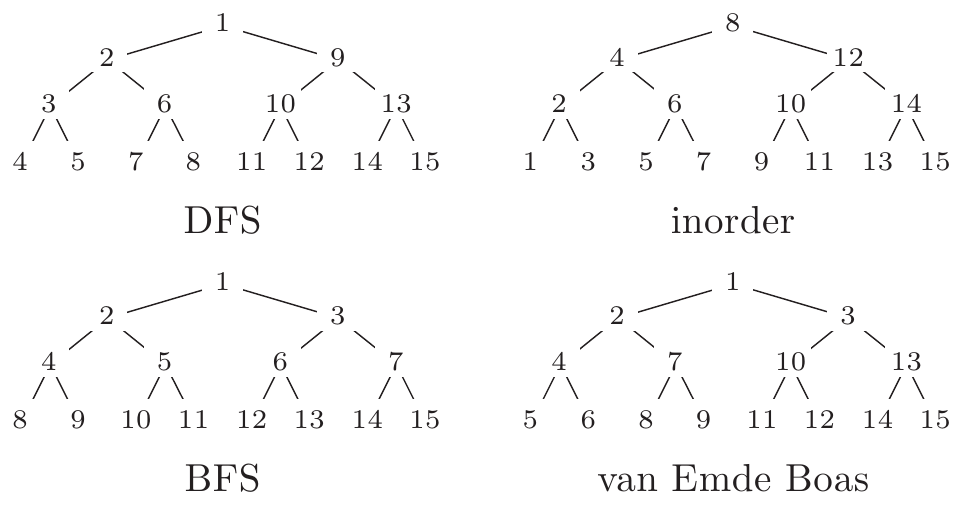
\includegraphics[width=\textwidth]{./Figures/Project1/MemoryLayouts.png}
		\rule{35em}{0.5pt}
	\caption[Memory layouts]{
	The four different tree structures shows the memory layout used in the implementations. The figure is taken from \citep{binAlg}.
	}
	\label{fig:memory_layouts}
\end{figure}


\subsection{Linear search}
To compare the running times for the algorithms, we have implemented a linear search function.
\begin{verbatim}
For each item in the list:
     if that item has the desired value,
         stop the search and return the item's location.
\end{verbatim}
 Return -1\footnote{We return -1 if the element dosn't exist in the list}.

\subsection{Inorder}

We have made a inorder binary search to compare with BFS, DFS and vEB.
Inorder is made iterative.
\lstinputlisting[language=C++, firstline=32, lastline=51, numbers=left]{./Figures/Project1/BinarySearch.cpp}
We begin by defining low, high and smallestSoFar.

In line 8 we make a while-loop, we run while high is greater than low.

We start by looking at the element whom is in the middle of the array.
If that element is smaller than the one we are looking for we set low to point at the middle +1.
If we are in the opposite case we set high to point at the middle -1.

The idea is that the array all the time is divided into one half the size where low will point at the first element in the new array and high will point at the last.

We continue until we find the element we are looking for or we return -1 if our list dosn't contain it.


\subsection{Breadth-first search (BFS)}


The following is a recursive method for filling out the bfs tree. The method is called by ``insert(0)''.
\begin{lstlisting}[numbers=left]
void insert(int bfsIndex){
  if (bfsIndex >= SIZE) return;
  insert(2*bfsIndex+1); // Left child
  bfsArray[bfsIndex] = *(linArray+linIndex);
  linIndex++;
  insert(2*bfsIndex+2); // Right child
}
\end{lstlisting}


The binary search is then implemented as follows:
\begin{lstlisting}[numbers=left]
  int i = 0;
  int curr = bfsArray[i];  // The current node visited
  int res = -1;  // The latest element smaller than 'elem'.
  while (curr != elem){
    i = 2*i+1;  // Left child
    if (curr < elem){
      i++;  // Right child (=left+1)
      res = curr;  // This is now the latest known element smaller than 'elem'.
    }
    // If we have reached a bottom node, return the last element lower than 'elem'.
    if (i >= SIZE){
      return res;
    }
    curr = bfsArray[i];
  }
  // At this point, the while loop did not continue because curr==elem
  return curr;
\end{lstlisting}



\subsection{Depth-first search (DFS)}
The implementation of depth first binary search (DFS) is based on \citep{binAlg}. 
The basic idea is to make a depth first traversal of the binary tree to create a different memory layout. 

The DFS implementation is build op like the other binary search implementations with a \verb!createDataStructure! and a \verb!binSearch! method. 
The \verb!createDataStructure! sets op the given sorted array in a DFS fashion and saves it in a new array, \verb!dfsArr!. 
The \verb!dfsArr! is created through a recursive method called \verb!dfsInsert!, that traverses the input array from left to right at insert in the \verb!dfsArr! in a recursive manner. 
The \verb!dfsInsert! method simulate traversal of the DFS tree and at each iteration of the tree-depth the method inserts the current element from the input array and then calls \verb!dfsInsert! on it's left and right children. 
\begin{lstlisting}[numbers=left]
void dfsInsert(int dfsIdx, int atDepth, int * inputArr) {
	if (dfsIdx < dfsArrSize && atDepth <= treeHeight) {
		int offset = floor(pow(2, (treeHeight - atDepth)));
		atDepth++;
		
		// Go left;
		dfsInsert(dfsIdx + 1, atDepth, inputArr);
		
		// Insert self	
		dfsArr[dfsIdx] = inputArr[insertFrom];
		insertFrom++;
		
		// Go right
		dfsInsert(dfsIdx + offset, atDepth, inputArr);
	}
} 
\end{lstlisting}
The left child is found by simply iterating one and the calculated \verb!offset! is used to find the left child. 
We observed that there is a relationship between two to the power of height of the tree and the current tree depth and index of the right child, 
and use this in the calculation of the offset.   

Making the actual binary search in the created DFS tree is done the same way as in the other algorithms, but also keeping track of the our current depth.
The highest value seen so far (lower than what we are looking for) is maintained and then the array is traversed like a binary tree. 
The main difference in DFS is what each time we need to visit the right child we calculate the \verb!offset! in same way as in \verb!createDataStructure!.  
But here shifting bits instead of using pow to save computation time (It could also been done this way in \verb!createDataStructure!, but we use \verb!pow! to ease the understanding). 
\begin{lstlisting}
 ...
// Go right
node = node + (1<<(treeHeight-atDepth));
...
\end{lstlisting}



\subsection{Van Emde Boas (vEB)}

The vEB array is constructed using the following recursive method. It is called using ``insert(0,0,0,roots)'' where roots is an array of the same size as the depth of the tree.

\begin{lstlisting}[numbers=left,escapeinside={@}{@}]
void insert(int vebIndex, int atDepth, int depthIndex, int roots[]){
  if (vebIndex >= size || vebIndex < 0) {
    return;
  }
  int rootIndex = findPosition((~atDepth+1) & atDepth); // returns the position of the rightmost 1-bit in "atDepth".
  int depthType = findPosition(~atDepth & (atDepth+1)); // returns the position of the rightmost 0-bit in "atDepth".
  int rootsNew[depth];
  for (int i=0; i<depth; i++){
      if (i <= rootIndex) rootsNew[i] = vebIndex;
      else rootsNew[i] = roots[i];
  }
  int amount = 1<<((1<<depthType)-1);  // 2^(2^depthType - 1)
  @\label{lst:vebLeft}@int vebLeft = (2*(depthIndex & (amount-1)) +1) * (2*amount -1) + rootsNew[depthType];  // (2*(depthIndex % amount)+1) * 2^(2^depthType) + "The root of the smallest local subtree"  insert(vebLeft, atDepth+1, 2*depthIndex, rootsNew); // Left child
  vebArray[vebIndex] = *(linArray+linIndex);
  linIndex++;
  int vebRight = vebLeft + 2*amount -1;
  insert(vebRight, atDepth+1, 2*depthIndex+1, rootsNew); // Right child
}
\end{lstlisting}

This vEB structure does not depend on the size of the input array. As a consequence, only inputs of size $2^{2^n}-1$ where $n$ is an integer generates fully balanced trees.
Otherwise it will always be more or less unbalanced, where the most of weight is located to the left. If for example the size is 9 then the left side will contain 7 elements compared to only 1 on the right side.
If we go one ``tree order'' further, if the size is 135, then there will be eight subtrees of size 15 each located to the of the root. That is, there will be 142 elements to the left of the root versus only 7 to the right.
In these two examples, almost half of the tree structure would not be utilized. Consequently, searching will on average require more iterations than balanced tree, since the tree is higher.
The worst case for this type of layout happens when the input size is $k 2^{2^n}$ where $2 < k \ll 2^{2^n}$. Then, more than half of the elements are located in the lower half of the tree, while at the same time, the tree is much higher than in a balanced tree.

The index calculation in line \ref{lst:vebLeft} is quite complex.
Some of the variables leading up to this calculation are illustrated in figure \ref{fig:vEB}.
\begin{figure}[htbp]
	\centering
		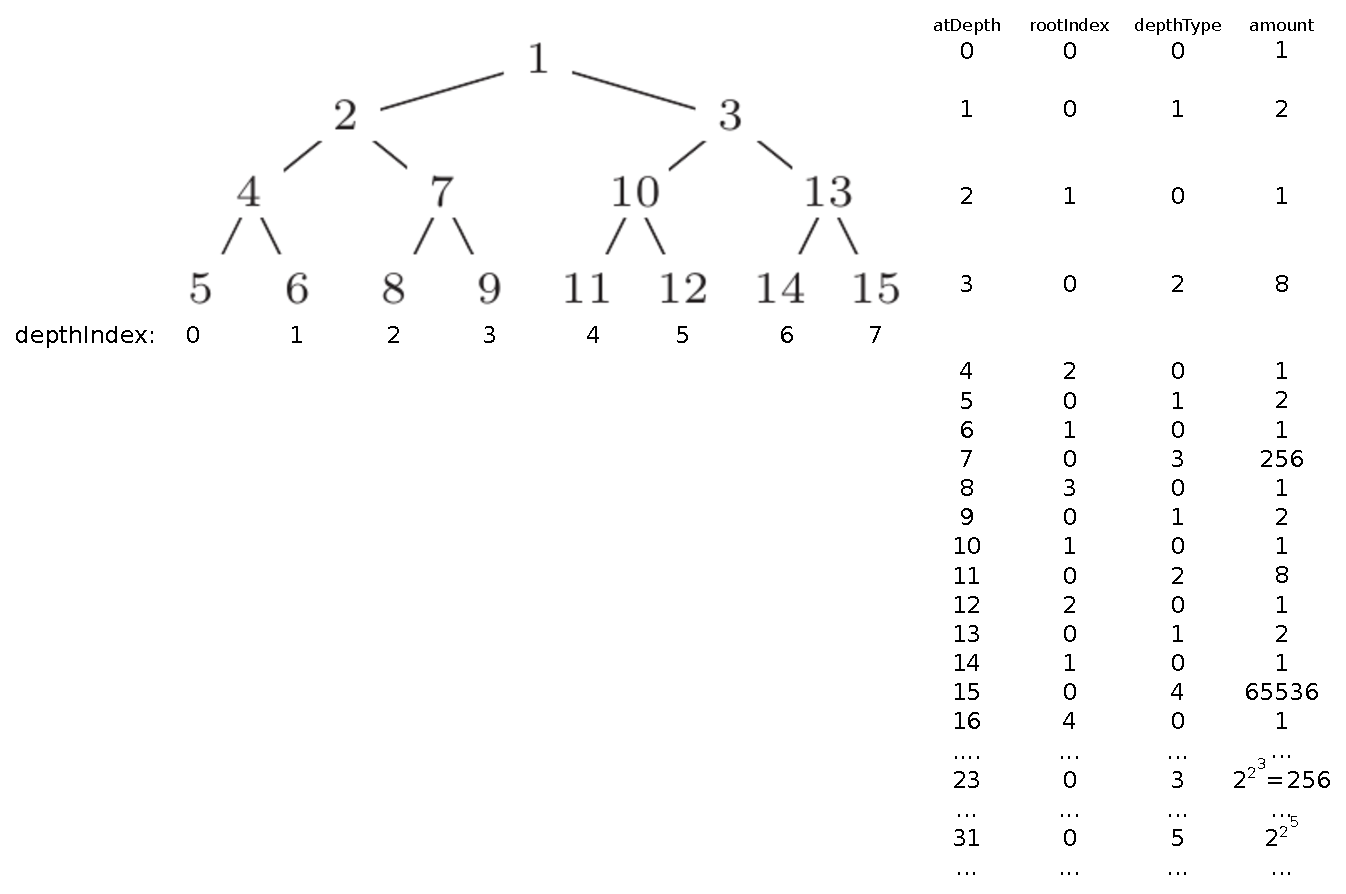
\includegraphics[width=\textwidth]{./Figures/Project1/vEB.eps}
		\rule{35em}{0.5pt}
	\caption[Van Emde Boas construction]{
	Bla bla bla.
	}
	\label{fig:vEB}
\end{figure}

First we do \verb!depthIndex&(amount-1)! which calculates how far to the right we are in the relevant subtree.
Then we double this value to find the number of new subtrees already placed by the neighbouring nodes to the left. One is added to take the current subtree into acount.
That value is now multiplied by the size of the current subtrees which is \verb!2*amount-1! to get the index of the left child in the parenting subtree.
Finally we add the index of root of the parenting subtree.


The binary search is implemented as follows:
\begin{lstlisting}[numbers=left]
  int vebIndex = 0;
  int curr = vebArray[vebIndex]; // The current node visited
  int res = -1; // The latest element smaller than 'elem'.
  int atDepth = 0;
  int depthIndex = 0;
  int roots[depth];
  for (int i=0; i<depth; i++){
      roots[i] = 0;
  }
  while (curr != elem){
    int rootIndex = ... // same as above
    int depthType = ...
    int amount = ...
    
    for (int i=0; i<=rootIndex; i++){
	roots[i] = vebIndex;
    }
    int goRight = curr < elem;
    vebIndex = (2*(depthIndex & (amount-1)) +1 + goRight) * (2*amount -1) + roots[depthType];

    if (goRight){
      res = curr;  // This is now the latest known element smaller than 'elem'.
    }
    if (vebIndex >= size || vebIndex < 0){
      return res;  // we have reached the bottom of the tree.
    }
    atDepth++;
    depthIndex = 2*depthIndex + goRight;
    curr = vebArray[vebIndex];
  }
  // At this point, the while loop did not continue because curr==elem
  return curr;
\end{lstlisting}








\section{Results and discussion}



\begin{figure}[htbp]
	\centering
		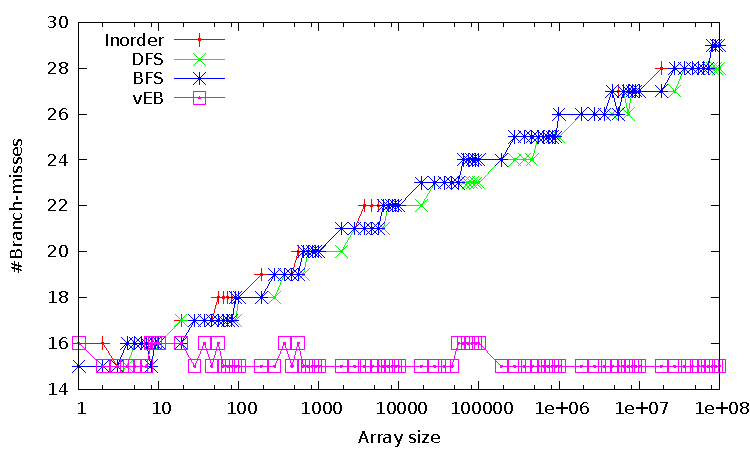
\includegraphics[width=\textwidth]{./Figures/Project1/Branch_misses.pdf}
		\rule{35em}{0.5pt}
	\caption[Branch misses]{
	Bla bla bla.
	}
	\label{fig:Branch_misses_p1}
\end{figure}


\begin{figure}[htbp]
	\centering
		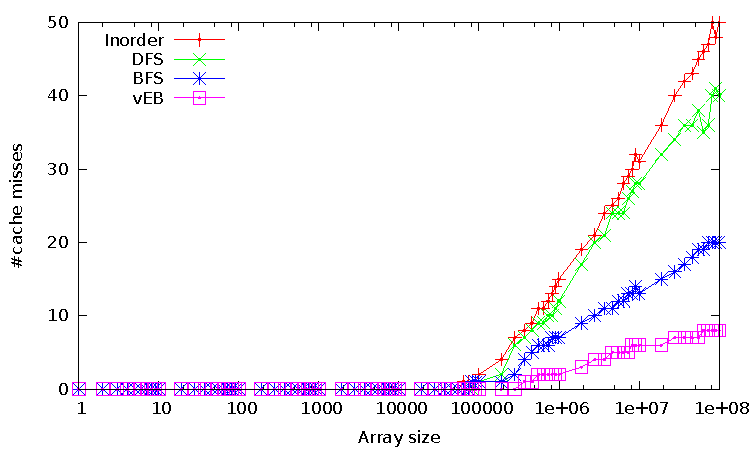
\includegraphics[width=\textwidth]{./Figures/Project1/Cache_misses.pdf}
		\rule{35em}{0.5pt}
	\caption[Cache misses]{
	Bla bla bla.
	}
	\label{fig:Cache_misses_p1}
\end{figure}



\begin{figure}[htbp]
	\centering
		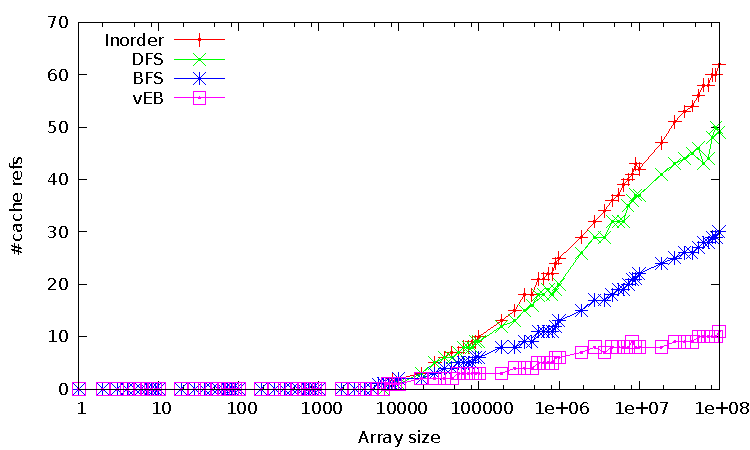
\includegraphics[width=\textwidth]{./Figures/Project1/Cache_refs.pdf}
		\rule{35em}{0.5pt}
	\caption[Cache refs]{
	Bla bla bla.
	}
	\label{fig:Cache_refs_p1}
\end{figure}



\begin{figure}[htbp]
	\centering
		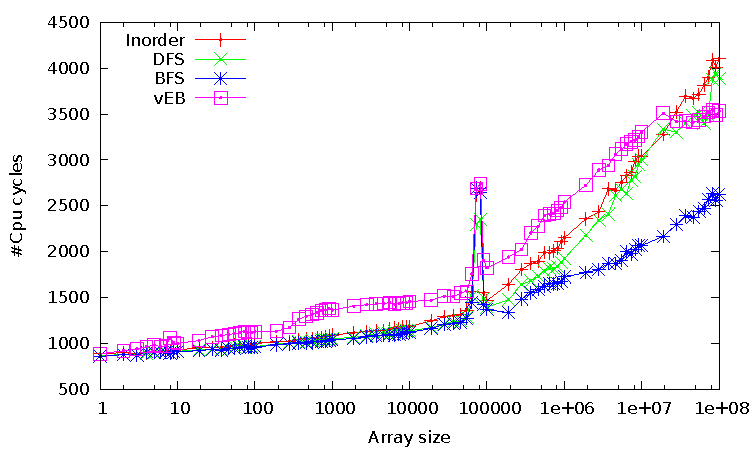
\includegraphics[width=\textwidth]{./Figures/Project1/Cpu_cycles.pdf}
		\rule{35em}{0.5pt}
	\caption[CPU cycles]{
	Bla bla bla.
	}
	\label{fig:Cpu_cycles_p1}
\end{figure}


\begin{figure}[htbp]
	\centering
		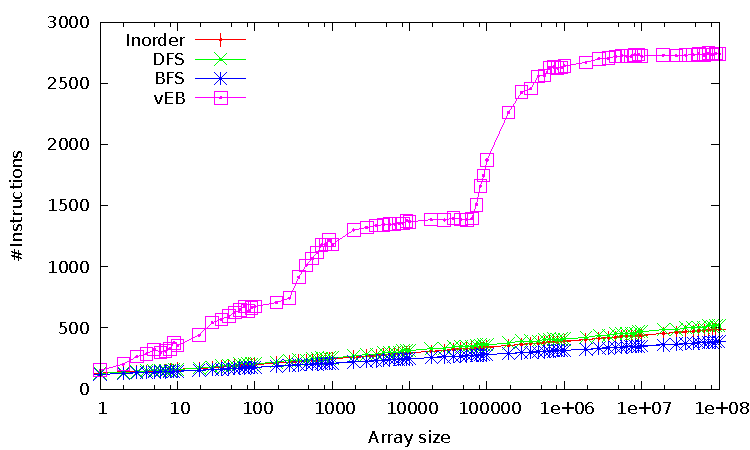
\includegraphics[width=\textwidth]{./Figures/Project1/Instructions.pdf}
		\rule{35em}{0.5pt}
	\caption[Instructions]{
	Bla bla bla.
	}
	\label{fig:Instructions_p1}
\end{figure}


% Chapter 2

\chapter{Project 2a: Matrix multiplication} % Main chapter title

\label{Chapter2} % for referencing this chapter elsewhere, use \ref{Chapter2}

\lhead{Chapter 2. \emph{Matrix multiplication}} % this is for the header on each page - perhaps a shortened title

%----------------------------------------------------------------------------------------


\section{Introduction}



\section{Implementations \citep{matrixMultiplication}}


\subsection{Naive Matrix Multiplikation}
We have implemented a naive matrix multiplication to compare with the other algorithms.

The first line creates a matrix for saving the result of the multiplication in.

Then for all the rows in the first matrix and all the colums in the second matrix we take sum of the row element multiplied with the column element for alle the elements in the current column and row.

Then we save the value in the resulting matrix.
After we have iterated trough all the columns and rows we return the resulting matrix.
\lstinputlisting[language=C++, firstline=16, lastline=29, numbers=left]{./Figures/NaiveMatrixMulti.cpp}

\subsection{Transposed}
\lstinputlisting[language=C++, firstline=5, lastline=6, numbers=left]{./Figures/Transpose.cpp}
We start by transposing the input matrix in a transpose method that is called in the setup method.
\lstinputlisting[language=C++, firstline=12, lastline=14, numbers=left]{./Figures/Transpose.cpp}
The setup method should always be called before the matrix multiplication method is used.
\lstinputlisting[language=C++, firstline=16, lastline=26, numbers=left]{./Figures/Transpose.cpp}
After the transpose method has been called we start by creating a matrix p we use to save the result in.
Then for all the colums in the transposed matrix mC, and all the colums in the second matrix B, we calculate the sum of the product between all the enties in the current column of mC and B.
When we have iterated through all the colums in both matrixes and saved the results we are done.
\lstinputlisting[language=C++, firstline=29, lastline=42, numbers=left]{./Figures/Transpose.cpp}


\subsection{Recursive}
The recursive multiplication is implemented as follows:
\begin{verbatim}
   int m = heightA;
  int n = widthA;
  int p = (*matrixB).nCols;
  B = matrixB;
  C = createMatrix(m, p);
  
  recMult(0, 0, 0, 0, m, n, p);
  
  return C;
\end{verbatim}

It makes use of the following recursive method:
\begin{verbatim}
void recMult(int i_A, int j_A, int i_B, int j_B, int m, int n, int p) {
  if (m==1 && n==1 && p==1) { // base case
    int AB = matrixGet(A, i_A, j_A)*matrixGet(B, i_B, j_B);
    matrixAdd(C, i_A, j_B, AB);
  } else if (m >= max(n,p)) { // split rows of A
    recMult(i_A,     j_A,     i_B,     j_B,     m/2,   n,     p    );
    recMult(i_A+m/2, j_A,     i_B,     j_B,     m-m/2, n,     p    );
  } else if (n >= max(m,p)) { // split columns of A and rows of B
    recMult(i_A,     j_A,     i_B,     j_B,     m,     n/2,   p    );
    recMult(i_A,     j_A+n/2, i_B+n/2, j_B,     m,     n-n/2, p    );
  } else if (p >= max(m,n)) { // split columns of B
    recMult(i_A,     j_A,     i_B,     j_B,     m,     n,     p/2  );
    recMult(i_A,     j_A,     i_B,     j_B+p/2, m,     n,     p-p/2);
  }
  return;
}
\end{verbatim}



\subsection{Tiled}
Idea:
The implementation of tiled matrix multiplication (TMM) is based on \citep{matrixMultiplication}, where TMM is presented as an example of an cache-aware algorithm. 
The approach is to multiply two matrices by dividing them into sub-matrices and multiplying these (see image). 
\begin{figure}[htbp]
	\centering
		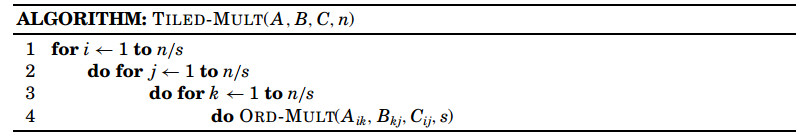
\includegraphics[width=\textwidth]{./Figures/Project2a/TiledMulti_Pseudo.jpg}
		\rule{35em}{0.5pt}
	\caption[Branch misses]{
	Bla bla bla.
	}
	\label{fig:Branch_misses}
\end{figure}
By doing this the idea is base the size of the sub-matrices on the cache size and thereby utilize the cache in the best way (i.e. fewer cache faults).   

Implementation:
TMM is implemented by splitting the input matrices (A and B) into S sub matrices in each dimension. Which in our case typically S = 4. 
Then each sub-matrix is calculated with the naive matrix multiplication method. 
The biggest challenge in the implemtation was to seperate the input matrices int sub-matrices without creating new matrices, which would use a lot of extra memory and computation time. 
Instead we keep track of the start indices og the sub-matrices and just access the input matrices to get the values. 
To keep track of how far we have gotten in each direction and in both A and B, and how big the next sub-matrices is, we keep updating six variables:
\begin{verbatim}
int subAnRows, subAnCols, subBnCols;
	int rowsVisitedA = 0;
	int colsVisitedA = 0;
	int colsVisitedB = 0;
\end{verbatim}
The size of the new sub-matrix (e.g. subAnRows) are updated each time we iterate in the corresponding direction (e.g. rows). 
The new value depends on how far we've gotten and the size of the input e.g.
\begin{verbatim}
subAnRows = ceil( (double) (A->nRows - rowsVisitedA) / (double) (s - i) );
\end{verbatim}
We only need three variables to maintain where we are in A and B and not four, because of the constraint that A has to have as many coloumns as B has rows for the two to be multiplied. 
Maintaining these values also means that A and B can be multiplied without depending on that they are symmetric or have the same size, as long as they comply with forementioned constraint.



\section{Results and discussion}



\begin{figure}[htbp]
	\centering
		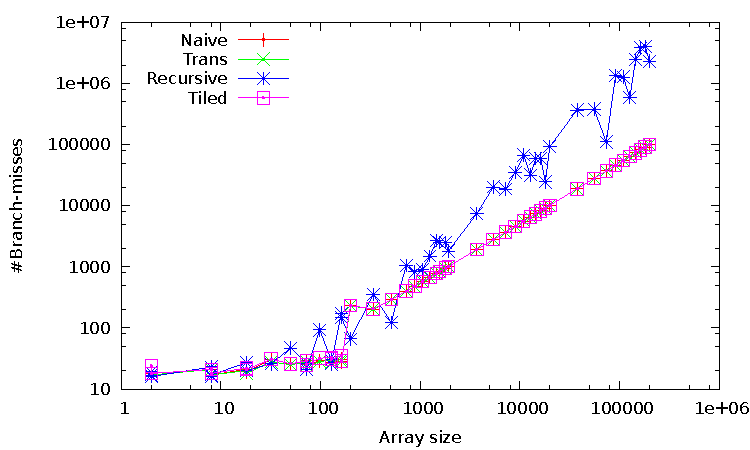
\includegraphics[width=\textwidth]{./Figures/Project2a/Branch_misses.pdf}
		\rule{35em}{0.5pt}
	\caption[Branch misses]{
	Bla bla bla.
	}
	\label{fig:Branch_misses}
\end{figure}


\begin{figure}[htbp]
	\centering
		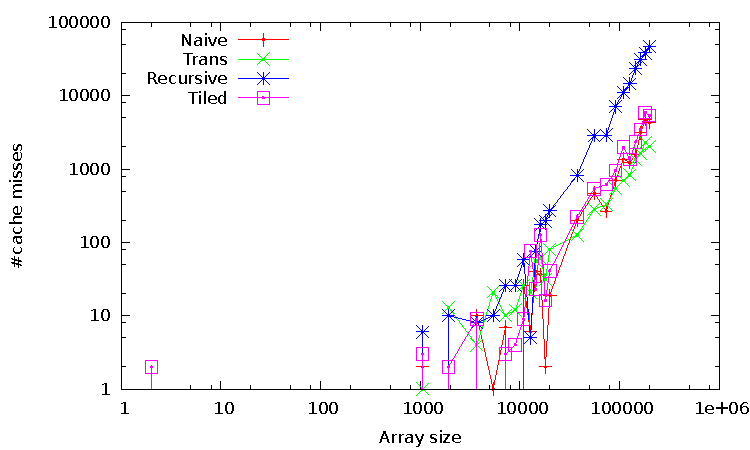
\includegraphics[width=\textwidth]{./Figures/Project2a/Cache_misses.pdf}
		\rule{35em}{0.5pt}
	\caption[Cache misses]{
	Bla bla bla.
	}
	\label{fig:Cache_misses}
\end{figure}



\begin{figure}[htbp]
	\centering
		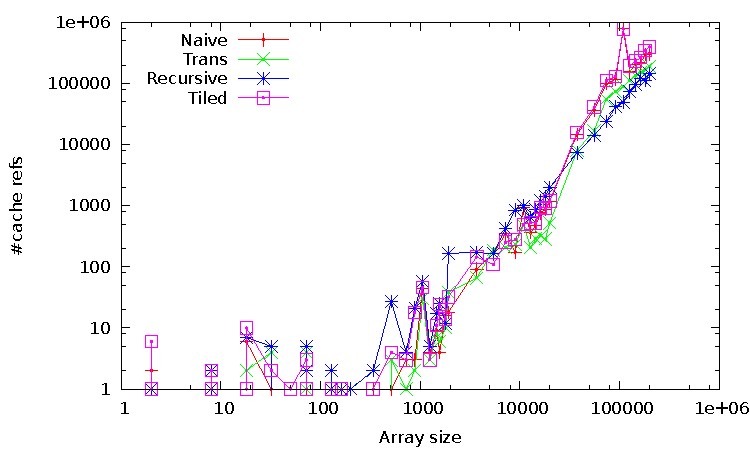
\includegraphics[width=\textwidth]{./Figures/Project2a/Cache_refs.pdf}
		\rule{35em}{0.5pt}
	\caption[Cache refs]{
	Bla bla bla.
	}
	\label{fig:Cache_refs}
\end{figure}



\begin{figure}[htbp]
	\centering
		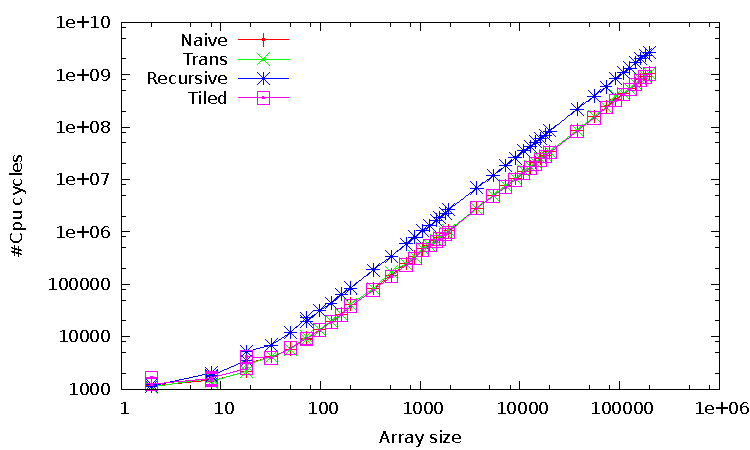
\includegraphics[width=\textwidth]{./Figures/Project2a/Cpu_cycles.pdf}
		\rule{35em}{0.5pt}
	\caption[CPU cycles]{
	Bla bla bla.
	}
	\label{fig:Cpu_cycles}
\end{figure}


\begin{figure}[htbp]
	\centering
		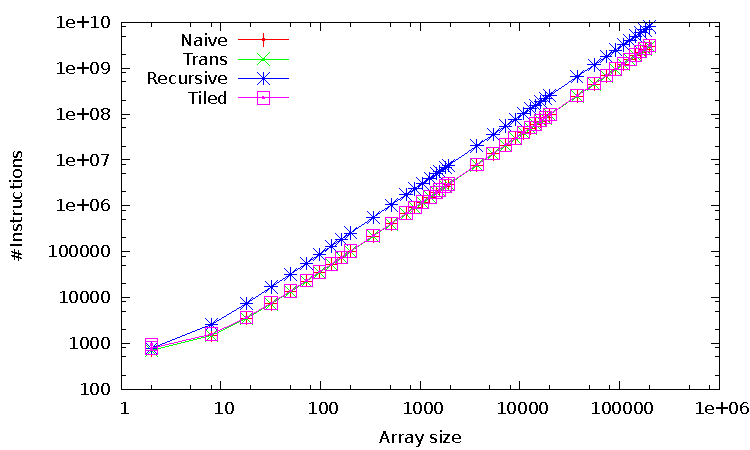
\includegraphics[width=\textwidth]{./Figures/Project2a/Instructions.pdf}
		\rule{35em}{0.5pt}
	\caption[Instructions]{
	Bla bla bla.
	}
	\label{fig:Instructions}
\end{figure}
 
% Chapter 3

\chapter{Project 2b: Radix sort} % Main chapter title

\label{Chapter3} % Change X to a consecutive number; for referencing this chapter elsewhere, use \ref{ChapterX}

\lhead{Chapter 3. \emph{Radix sort}} % Change X to a consecutive number; this is for the header on each page - perhaps a shortened title

%----------------------------------------------------------------------------------------


\section{Implementations}
This project describes experiments done with different sorting algorithms for sorting arrays of int keys. The implementations centers around radix sort, but we also perform experiment with QuickSort and CountingSort to have something to compare with.
All algorithms in this project is based on approaches in \citep{radixSort}.
The implementations have two methods:
\begin{lstlisting}
  void setup(int arrSize);
  int* sort(int* array, int arrSize);
\end{lstlisting}
\verb!setup! is used to set up the algorithms and \verb!sort! sorts the array, which is the only one we measure in our experiments.

The algorithms that sort based on digits, all assume that a digit, D, is 8 bits and the size of an int, K, is 32 bits.
The goal of this project is to implement a Multi-core Radix Sort which uses both Most Significant Digit (MSD) - and Lowest Significant Digit (LSD) Radix Sort, and compare this implementation with other relevant sorting algorithms.


\subsection{Counting sort (CS)}
We start by finding the greatest value in the list gKey.
gKey = Max(Array)+1
We use gKey to create a new array C and for every entry in C we set the value to 0.
in line 4-5 we go through the input array and use the Histogram array to keep trak of how many of a specific element we have, so for all the elements in array we go to the equvalent index in Histogram and increase it by 1.
In line 6-7 we use the Histogram to calculate the starting index of each key in array.
In the last loop we go through the Histogram array and we iterate from the last index and down to the beginning of the array.
The index of Histogram[array[j]-1] is where the j'th element of array should be in the result array.
Then we count down the Histogram[array[j]] by 1.
This work for the case where we have multiple of the same key and in the case where we have only one of each key, because in line 11 we decrease the starting index by 1 after having placed one instance of the key, so the previous won't be overwritten.
\lstinputlisting[language=C++, firstline=32, lastline=46, numbers=left]{./Figures/Project2b/CountingSort.cpp}


\subsection{Quick sort (QS)}
We use a Quick Sort from a \verb!C++! library because we want to compare our other algorithms with one that has a running time of $ O(n\cdot \log n) $ which Quick Sort does.
We call the library function in line 1 which takes an array, the size of the array, the type of elements (int in our case) and a compare function.
\lstinputlisting[language=C++, firstline=20, lastline=21, numbers=left]{./Figures/Project2b/QuickSort.cpp}
The compare function states that the input should e sorted from the smallest key to the greatest.
\lstinputlisting[language=C++, firstline=13, lastline=16, numbers=left]{./Figures/Project2b/QuickSort.cpp}


\subsection{Least significant digit (LSD)}
To have something to compare the Multi-core Radix Sort to, we implemented, among others, Least Significant Digit (LSD) radix sort. 
The idea is to sort the input array of keys into buckets starting from the lowest significant digit. After each sorting into buckets for a digit an array sorted from the that digit is produced. 
This is done for each digit until the input array is fully sorted. 

The implemtation uses C++ \verb!std:queue! structure to simulate buckets. We assume that this data structure utilizes memory and computation quite effectively, and it seem logical to use this instead of creating our own bucket data structure.
In the method 'sort' the pgram sorts the array as mentioned before, by iterating over the digits starting from the lowest significant one. At each iteration sorting the keys into buckets and then creating a new array from these buckets.
\begin{lstlisting}[numbers=left]
...
for (int i = 0; i < N_PASSES; i++) {
  for (int j = 0; j < arrSize; j++) {
    // Add to bucket
    buckets[ (sortedArray[j] >> (K-i*D)) & MASK_D ].push(sortedArray[j]);
  }
  // Create sorted array from buckets
  int sortArrIdx = 0;
  for (int k = 0; k < N_BUCKETS; k++) {
    while(!buckets[k].empty()) {
      sortedArray[sortArrIdx] = buckets[k].front();
      buckets[k].pop();
      sortArrIdx++;
    }
  }
}
\end{lstlisting}
\verb!sortedArray[j] >> (K-i*D)) & MASK_D! gets the digit we want to look at by right shifting the value and anding it with a bit mask containing 0s except for the lowest D bits, which is 1s.

The algorithm was straight forward to implement an contains no complex computation. If one wanted to improve performance a differen datastructure for buckets could maybe be used.



\subsection{Most significant digit (MSD)}
MSD radix sort is very similar to LSD. However, we now sort the input by looking at the digits in descending order.
After distributing the elements in buckets according to the most significant, these buckets are then sorted recursively.

The MSD radix sort is implemented as follows:
\begin{lstlisting}[numbers=left]
  // Pass 0
  queue<int> buckets[N_BUCKETS];
  for (int i = 0; i < arrSize; i++) {
    // Add to bucket
    buckets[ sortedArray[i] >> (K-D) ].push(sortedArray[i]);
  }
  // Pass 1 (and the rest, recursively)
  for (int b = 0; b < N_BUCKETS; b++) {
    msdRecursive(buckets[b], 1);
  }
  return sortedArray;
\end{lstlisting}

It makes use of the following recursive method:
\begin{lstlisting}[numbers=left]
void msdRecursive(queue<int> bucket, int pass) {
  if (bucket.empty()) return;
  
  // Base case (this bucket is already fully sorted).
  if (pass == N_PASSES) {
    while(!bucket.empty()) {
      sortedArray[sortArrIdx] = bucket.front();
      bucket.pop();
      sortArrIdx++;
    }
    return;
  }
  // Sort this bucket into some new buckets.
  queue<int> buckets[N_BUCKETS];
  while(!bucket.empty()) {
    const int key = bucket.front();
    bucket.pop();
    // Add to bucket
    buckets[ (key >> (K - (pass+1)*D)) & MASK_D ].push(key);
  }
    // Example (K=8, D=2, pass=1, so we have already sorted by AB, and now we look at CD):
    // (ABCDEFGH >> (8 - (1+1)*2)) & 00000011
    // (ABCDEFGH >> 4) & 00000011
    //  0000ABCD & 00000011
    //  000000CD

  // Now, sort all buckets recursively.
  for (int b = 0; b < N_BUCKETS; b++) {
    msdRecursive(buckets[b], pass+1);
  }
}
\end{lstlisting}

\subsection{MSD - using arrays (MSD\_arr)}
This version of MSD radix sort makes use of one long array for each digit to by.
These arrays are then of length \verb!N_KEYS*N_BUCKETS!. When we choose the number of buckets to be $2^8=256$, this would conceivably use that much more memory.
However, when we only declare the arrays without initializing, the paged virtual memory can handle this kind of array by mapping the physical memory only when the pages are first accessed \citep{radixSort}.


\subsection{Multicore radix sort (MCR)}
The implementation of Multi-core Radix Sort (MCR) is based on the approach in \citep{radixSort}. The idea behind is to use the benefits of both MSD and LSD and making the algorithm parallel to decrease computation time. 
The algorithm first partitions the input array into buckets with based on MSD and then sort each of theses buckets locally with using LSD.  
MSD has the disavangtage of not being very effective on arrays of small size or values is close to each other, because it can results of a lot of empty buckets. 
But has the advantage that when values have the same digit these doesn't have to be moved around. LSD on the other hand will have to move values that share prefix around again and again.
LSD has the advantage of handling non-uniform distribution of values better than MSD, but has the tradeoff of copying data around.  

The implementation is based on the pseudocode from the forementioned article:
\begin{figure}[htbp]
	\centering
		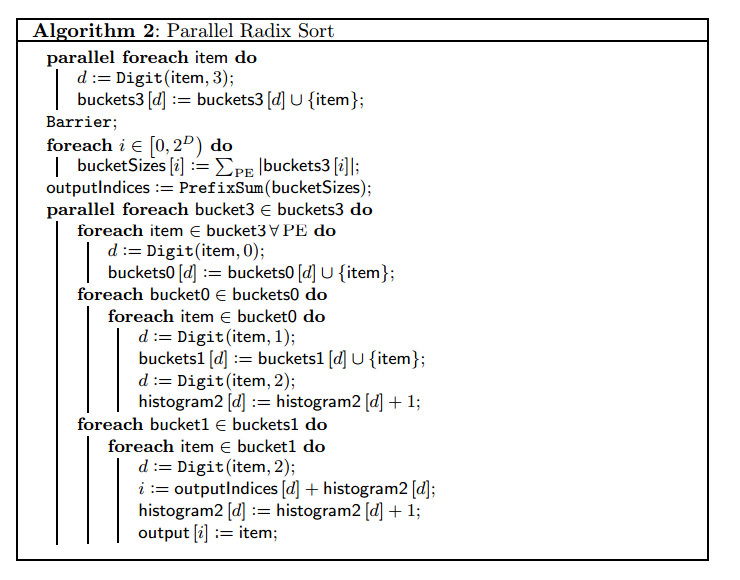
\includegraphics[width=\textwidth]{./Figures/Project2b/MultiCoreRadix_Pseudo.jpg}
		\rule{35em}{0.5pt}
	\caption[Multicore radix pseudocode]{
	Pseudocode for Multi-core Radix Sort
	}
	\label{fig:Branch_misses}
\end{figure}
As in the pseudocode the program starts out by sorting the array based on the most significant digit in parallel, then serial compute output indicies (PrefixSum in the pseudocode) and finally parallel sort each bucket based on LSD.  
The parallel parts is implemented using POSIX threads (\verb!<pthread.h>!), which by default utilizes multicore cpus by starting each thread on a new cpu.

The program has two 2D arrays which respectively holds buckets and bucket histograms for each thread. These are called threadBucketArrays and threadNextArrays.
Each of the bucket arrays in threadBucketArrays inititally took up N x M space, where N is elements in the input array and M is number of buckets.
This means a lot of space had to be reserved by the program. To minimize this space usage, N is bound by the number of elements assigned to the current thread.
This yields that each bucket array takes up (N / P) x M, where P is the number of threads. 

The parallel MSD part (first part) assigns part of the input array to each thread, which then sort the elements int buckets based on the most significant digit.
The sorting is saved in the formentioned shared threadBucketArrays using threadNextArrays to index these bucket arrays:
\begin{lstlisting}
...
bucketArray[ putInBucket*nElemsAssigned[tInfo->threadNum] + nextArray[putInBucket] ] = inputArray[i];
nextArray[putInBucket]++; 
... 
\end{lstlisting}
bucketArray and nextArray coresponds to the threads arrays in threadBucketArrays and threadNextArrays.

The next part consist of the program computing (serial) output indices used to index the output array by traversing over the all the threads nextArrays.   
The array computed from this, ouputMSDStartIndices, is a kind of prefix sum over sizes of the MSD-bucket, but where the values are shifted on to the right in the array (i.e. the first element is 0).

In the last part, the MSD buckets is divided among the threads, which sort the assigned buckets locally based on LSD and then write sorted values to the output array.
For each MSD bucket assigned to a thread, it first sort the values in the bucket into new buckets (locally) based on the lowest significant digit. This is straight forward.
Then traversing through the bucket sorted by lowest significant digit, the values are divided into buckets depending on the second lowest significant digit.
And in same traversal a histogram for the third lowest significant digit is produces.
\begin{lstlisting}
...
  for (int bucket = 0; bucket < nBuckets; bucket++) {
    for (int i = 0; i < nexts0[bucket]; i++) {
      elem = buckets0[bucket*arraySize + i];

      // Put in bucket
      putInBucket = (elem >> shiftRight2nLast) & lsdBitMask;
      buckets1[putInBucket*arraySize + nexts1[putInBucket]] = elem;
      nexts1[putInBucket]++;

      // Histogram
      histIdx = (elem >> shiftRightLast) & lsdBitMask;
      histogram2[histIdx]++;
    }
  }
...
\end{lstlisting}
This histogram is then used to produce a prefix sum following same procedure as for the output indices.
\begin{lstlisting}
... 
  prefixSum2[0] = 0;
    for (int i = 0; i < nBuckets; i++) {
      // Prefix sum
      if (i != nBuckets -1) {
	prefixSum2[i+1] = prefixSum2[i] + histogram2[i];
      } 
  }
...
\end{lstlisting}

This prefix sum is used together with the calculated output indices (\verb!ouputMSDStartIndices!) to index the sorted values to the correct positions int the output array.
\begin{lstlisting}
...
  // Last pass: write to output array
  for (int bucket = 0; bucket < nBuckets; bucket++) {
    for (int i = 0; i < nexts1[bucket]; i++) {
      elem = buckets1[bucket*arraySize + i];

      putInBucket = (elem >> shiftRightLast) & lsdBitMask;

      outputIdx = startIdxForMSDBucket + prefixSum2[putInBucket];

      prefixSum2[putInBucket]++;
      sortedArray[outputIdx] = elem;
    }
  }
... 
\end{lstlisting}
Where \verb!startIdxForMSDBucket = ouputMSDStartIndices[msdBucket]!.
This trick by using the computed prefix sum for the third lowest significant digit, saves a traversal of the buckets and makes the algorithm a bit faster.

The program uses hardcoded D and K, where D is number of bits per digit and K is number of bits per integer. Our implementation assumes that these values always is K = 32 and D = 8.
The implementation could be made generic, taking an abitrary K and D, but we didn't have the time and the algorithm in the article is depends on these values of D and K.
A generic solution could be achieved simply by adding LSD sorting in between the first LSD sorting and the second to last LSD sorting.

It turns out that the parallel parts of this implementation in fact doesn't run in parallel. This is with high probability because some methods locks the program to make serial computation.
We now for a fact that the \verb!srand! methods does this, but what other functionality in the implementation has this effect.   

\begin{figure}[htbp]
	\centering
		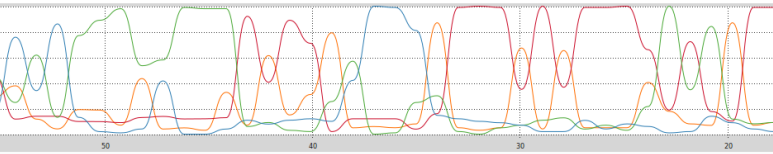
\includegraphics[width=\textwidth]{./Figures/Project2b/multicore_cpu_usage.png}
		\rule{35em}{0.5pt}
	\caption[Multicore CPU usage]{
	MCR threads running in serial.
	}
	\label{fig:multicore_cpu_usage}
\end{figure}

As seen in figure \ref{fig:multicore_cpu_usage}, different threads on different cpus is started, but these doesn't run in parallel.

\section{Results and discussion}


\begin{figure}[htbp]
	\centering
		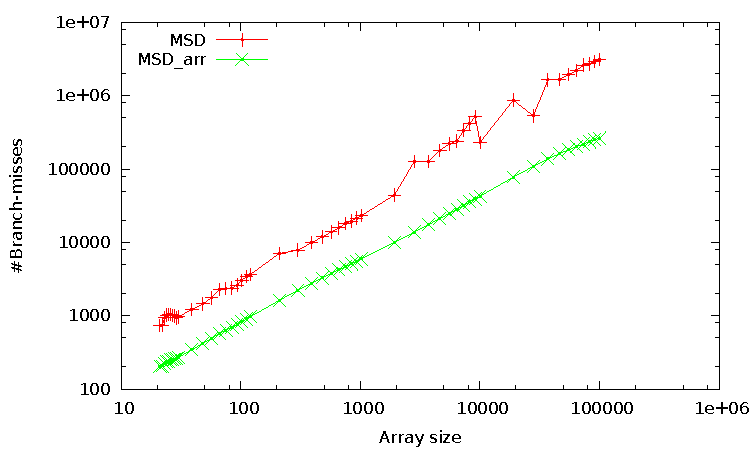
\includegraphics[width=\textwidth]{./Figures/Project2b/Branch_misses.pdf}
		\rule{35em}{0.5pt}
	\caption[Branch misses]{
	Branch misses for sorting algorithms based on array size.
	}
	\label{fig:Branch_misses_p2b}
\end{figure}

\begin{figure}[htbp]
	\centering
		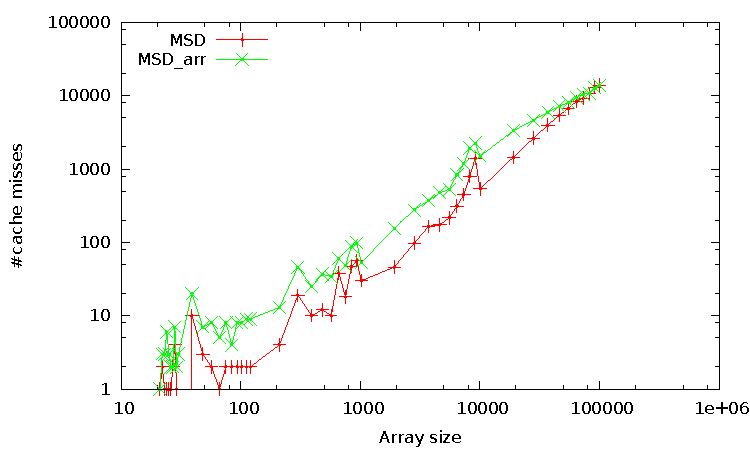
\includegraphics[width=\textwidth]{./Figures/Project2b/Cache_misses.pdf}
		\rule{35em}{0.5pt}
	\caption[Cache misses]{
	Cache misses for sorting algorithms based on array size.
	}
	\label{fig:Cache_misses_p2b}
\end{figure}




\begin{figure}[htbp]
	\centering
		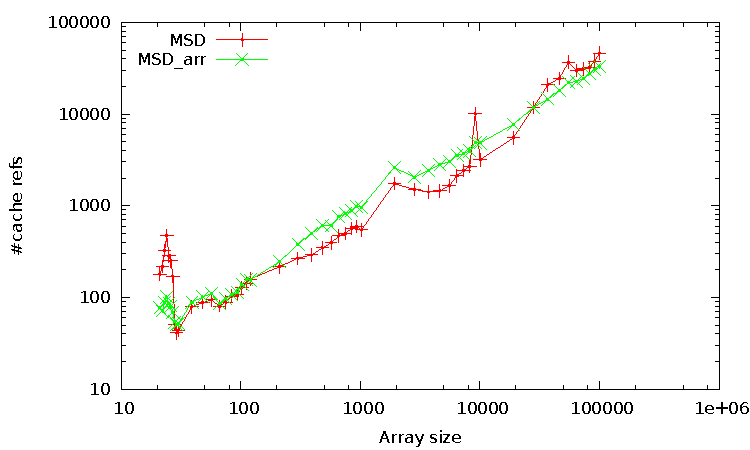
\includegraphics[width=\textwidth]{./Figures/Project2b/Cache_refs.pdf}
		\rule{35em}{0.5pt}
	\caption[Cache refs]{
	Number of cache references for sorting algorithms based on array size.
	}
	\label{fig:Cache_refs_p2b}
\end{figure}



\begin{figure}[htbp]
	\centering
		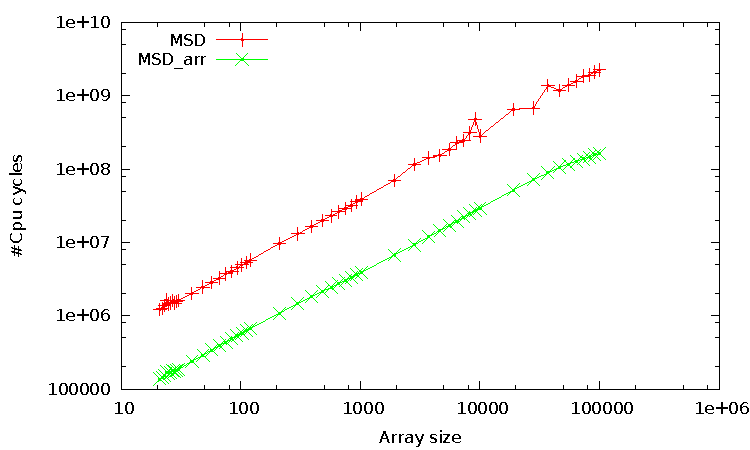
\includegraphics[width=\textwidth]{./Figures/Project2b/Cpu_cycles.pdf}
		\rule{35em}{0.5pt}
	\caption[CPU cycles]{
	Measure CPU cycles for sorting algorithms based on array size.
	}
	\label{fig:Cpu_cycles_p2b}
\end{figure}


\begin{figure}[htbp]
	\centering
		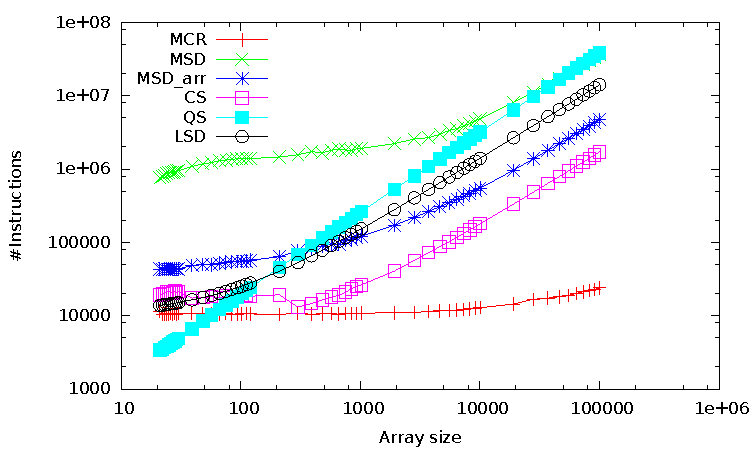
\includegraphics[width=\textwidth]{./Figures/Project2b/Instructions.pdf}
		\rule{35em}{0.5pt}
	\caption[Instructions]{
	Hardware instructions for sorting algorithms based on array size.
	}
	\label{fig:Instructions_p2b}
\end{figure}
The algorithm that using fewest instructions is MCR, which at first glance seems surprising for such a complex algorithm.
MCR also has the lowest gradient where QS has the steepest, which maybe could be explained by the recursive manner of QuickSort.
Logically the slope MCR should follow LSD and/or MSD, because MCR uses approach from both of them.
A guess to the low number of instructions for MCR, could be that a lot of instructions can be optimized away.
The algorithm with the highest number of base instructions is MSD, which can be explained by that a lot of queue is created in the recursive structure wchich all needs to be maintained. 

\begin{figure}[htbp]
	\centering
		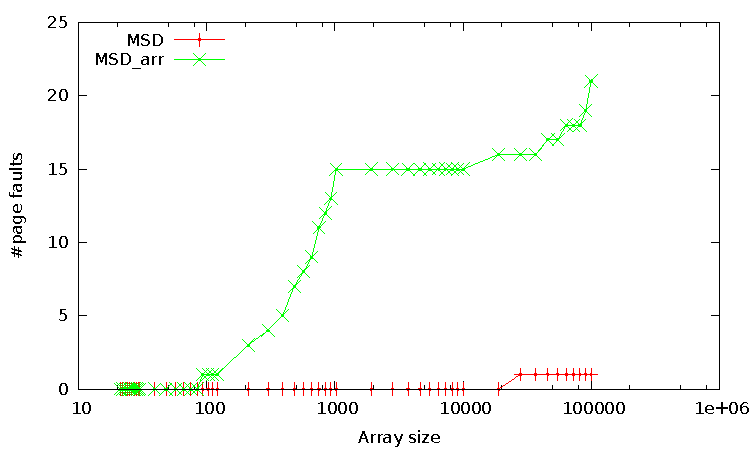
\includegraphics[width=\textwidth]{./Figures/Project2b/Page_faults.pdf}
		\rule{35em}{0.5pt}
	\caption[Page faults]{
	Memory page faults for sorting algorithms based on array size.
	}
	\label{fig:Page_faults_p2b}
\end{figure}



%\input{./Chapters/Chapter4} 
%\input{./Chapters/Chapter5} 
%\input{./Chapters/Chapter6} 
%\input{./Chapters/Chapter7} 

%----------------------------------------------------------------------------------------
%	THESIS CONTENT - APPENDICES
%----------------------------------------------------------------------------------------

%\addtocontents{toc}{\vspace{2em}} % Add a gap in the Contents, for aesthetics

%\appendix % Cue to tell LaTeX that the following 'chapters' are Appendices

% Include the appendices of the thesis as separate files from the Appendices folder
% Uncomment the lines as you write the Appendices

%% Appendix A

\chapter{Appendix Title Here} % Main appendix title

\label{AppendixA} % For referencing this appendix elsewhere, use \ref{AppendixA}

\lhead{Appendix A. \emph{Appendix Title Here}} % This is for the header on each page - perhaps a shortened title

Write your Appendix content here.
%\input{./Appendices/AppendixB}
%\input{./Appendices/AppendixC}

%\addtocontents{toc}{\vspace{2em}} % Add a gap in the Contents, for aesthetics

\backmatter

%----------------------------------------------------------------------------------------
%	BIBLIOGRAPHY
%----------------------------------------------------------------------------------------

\label{Bibliography}

\lhead{\emph{Bibliography}} % Change the page header to say "Bibliography"

\bibliographystyle{unsrtnat} % Use the "unsrtnat" BibTeX style for formatting the Bibliography

\bibliography{Bibliography} % The references (bibliography) information are stored in the file named "Bibliography.bib"

\end{document}  